\section{Experiment Description}

%The test problem(s) used in the experiments.
\subsection{Test Problems}
In Dr. Craig McGowan's research, a \textbf{Simulated Annealing (SA)} algorithm
is used. SA's are superior for some statistical problem over conventional 
algorithms \cite{goffe-sa}, like optimizing muscle excitation patterns. 
SA's are modeled after the method used to cool and
harden material like steel.
The start with a high 'temperature', which in optimization resembles the cost / 
error level of solution parameters. The temperature is decreased by picking 
random neigbor solutions that are better or worse within a certain tolerance.
This tolerance is relative to the temperature, and as time passes and the 
temperature decreases, the tolerance becomes less.

The temperature is measured on how well muscle excitation pattern solutions
simulate walking. Walking is judged on a fitness function, described in 
section \ref{sec:fitness}.

%A description of the evolutionary algorithm used in the experiments.
\subsection{Genetic Algorithm}
To start, we wanted to start with a GA that was as similar to an SA baseline 
as possible. The GA could then be varied, trying different methods with 
increasing variation. This first approach was to use a GA with a 
\textbf{generational} method of regeneration, a \textbf{tournament selection} 
method for crossover, a \textbf{flip or two point crossover} method, and a 
modified 
\textbf{uniform mutation} for newly generated individuals.

A Genetic Algorithm (GA) creates a \textbf{population} of individuals, each of which have attributes to try to solve a problem. Their correctness will be measure with a \textbf{fitness function}. The best of these individuals are found with \textbf{selection}, their attributes are combined using \textbf{crossover}, and a child is produced from this. Each child is then slightly \textbf{mutated}, or its attributes changed. This results in new individuals in the population, and the whole process is started again.

Please note that in this report, \textbf{max fitness is the worst}, and 
\textbf{min fitness is the best}. This is non-intuitive, because usually 
$ fitness = \frac{1}{cost} $. But this project used $ fitness = cost $ for 
technical reasons.

The \textbf{population} for all the GA methods in this report is represented as a list of vectors. The \textbf{initial population} has random values set in the attributes vector (x) for every individual (see Figure \ref{uniform_mutation}):
\begin{figure}[!h]
	\begin{center}
		\begin{tabular}{r l}
		$ P = i_1, i_2, ... i_j $& \\
					& where \\
					& $ i_n $ is a vector of floats or integers ( $ = x_1, x_2, ... x_y $ ) \\
					& $ j = 10 $ \\
					& $ y = 96 $ \\
					& $ x_n = [B_L, B_U] $ \\
					& $ B_L $ is the lower bound, $ = -5.0$ \\
					& $ B_U $ is the upper bound, $ = 100.00$\\
		\end{tabular} 
               	\caption{The representation of the population}
                \label{population}
        \end{center}
\end{figure}

\subsubsection{Selection}
For \textbf{tournament selection} (Figure \ref{selection}), the two individuals with the smallest fitnesses (best) will be selected from a random sample of the entire population. The sample size is represented by $ k $. As $ k $ gets bigger, the best individuals of a population are more likely preserved, while $ k $ getting smaller means more variety in the population. 
\begin{figure}[!h]
        \begin{center}
		\begin{tabular}{r l}
			$ selection(P) = $ &$ i_1, i_2, ... i_k$ \\
					& \\
					& where \\
					& $ P $ is the entire population \\
					& $ i_k $ is a random individual \\
					& $ k $ is the sample size, specified at run time \\
		\end{tabular} 
               \caption{The selection function}
                \label{selection}
        \end{center}
\end{figure}

Generally, $ k $ being larger leads to conversion on local optimums that the population may be surrounding, while $ k $ being lower allows individuals that may lead to some other optimum to remain. 

\subsubsection{Crossover}
The \textbf{crossover} function will take two individuals $ i_a, i_b $, and return a child individual, which has a mix of attributes ( $x_n $ values) from each parent. 

One crossover method we may use is \textbf{two point crossover}:
\begin{figure}[!h]
        \begin{center}
		\begin{tabular}{r l}
	                $ crossover(i_a, i_b) = $ & \\
			& $ x_{i_a}[1:n], x_{i_b}[n + 1:m], x_{i_a}[m + 1:length(x_{i_a})] $ x values for the new child individual \\
			& where \\
			& $ n = $ a random integer from $ 1 ...  m - 1 $ \\
			& $ m = n + 1 $ the length of $ x_{i_a} $ or $ x{i_b} $ (same) \\
		\end{tabular} 
               	\caption{Two point crossover}
                \label{two_crossover}
        \end{center}
\end{figure}

Another crossover method may be \textbf{flip crossover}, where $ n $
attributes are swapped between two different individuals:

\pagebreak

\subsubsection{Uniform Mutation}
Uniform mutation takes $ k $ values in an individual and sets them to new
random values:

\begin{figure}[!h]
        \begin{center}
		\begin{tabular}{r l}
		$ mutate(x_i) $ & $ = x_{i}{'}[a_1,a_2, ... a_n] $  \\
				& where \\
				& $ k $ attributes $ a_1, a_2... $ are mutated by setting them to $ f(a_x)  $ \\
				& $ f(a_x) = a_x + ( (a_x + m) * scale ) $ \\
				& $ m = $ random value between $ B_L $ and $B_U$ \\
				& $ B_L $ is the lower bound, $ = -5.0$ \\
				& $ B_U $ is the upper bound, $ = 100.00$ \\
				& $ k = 1 $ \\
				& $ scale = \frac{1}{800}$ 
		\end{tabular} 
               	\caption{Uniform mutation}
                \label{uniform_mutation}
        \end{center}
\end{figure}

\subsubsection{Generational Reproduction}
Generation reproduction of the population happens every cycle. It consists of
selection, crossover, and mutation mentioned in the sections previously.The 
flow of converging on a solution is as follows:
\begin{itemize}
	\item while user doesn't quit the process
	\begin{itemize}
		\item calculate current fitnesses
		\item select 2 individuals (parents) with minimum (best) fitnesses from a random subset of the entire population
		\item create new child from the 2 parents using crossover
		\item mutate the new child using uniform mutation
		\item replace the the max fitness individual (worst), with the new child
	\end{itemize}
\end{itemize}

\pagebreak
%How fitness was measured.
\subsection{Fitness Function}
\label{sec:fitness}
The fitness function is the cost function provided by Dr. McGowan's research:
\begin{figure}[!h]
        \begin{center}
                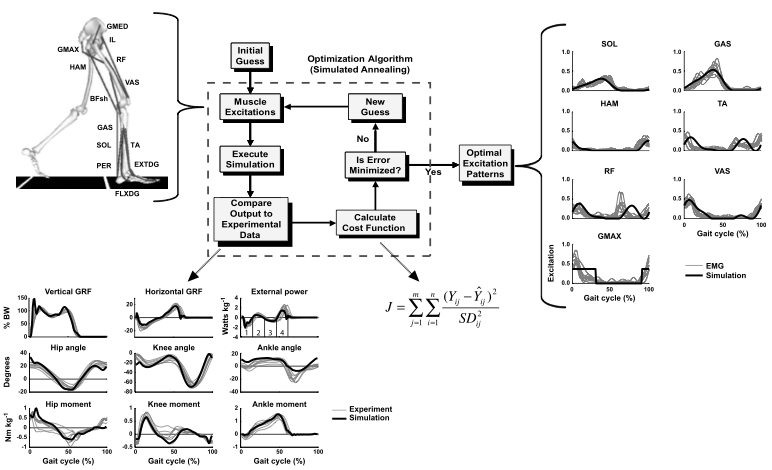
\includegraphics[width=130mm]{images/fitness_func}
                \caption{Fitness function overview \cite{mcgowan-fit}}
                \label{fitness_func_pic}
        \end{center}
\end{figure}
\pagebreak

%What parameters were used.
\subsection{Parameters}
The parameter POP\_SIZE is the population size. It is set to 10 for all 
experiments.

ATTR\_SIZE is how many attributes each individual has. It is set to 96 for all
experiments.
	
GA\_LBOUND is the lower bound for random mutation values. It is set to
-5.000 for all experiments.

GA\_UBOUND is the upper bound for random mutation values. It is set to 
100.00 for all experiments.

GA\_DIFF\_SCALE is the $ scale $ value in Figure \ref{uniform_mutation}. It
is set to 800.000 for all experiments.

K\_MUT is the denominator to equation $ k = \frac{population size}{K\_MUT} $, 
where $ k $ is in Figure \ref{uniform_mutation}. It is set to 96 for all
experiments.

K\_SELECT is the denominator to the equation 
$ k = \frac{population size}{K\_SELECT} $, $ k $ belonging to Figure 
\ref{selection}. It is set to 1 for all experiments.

K\_FLIP\_XOVER is the number of points to flip in flip crossover.

%An clear explanation of how the results would support, or refute, the hypothesis. You should be able to say, before running any experiments, 'if I get these set of results it means the hypothesis is confirmed (or at least supported) and if I get this set of results the hypothesis is refuted'.
